\documentclass{article}

\usepackage{listings}
\usepackage{graphicx}

\title{Notes on Supercomputing with Hyak}
\author{M.P.Ross}

\begin{document}
\maketitle
\section{Parallel Computing}
There are two main types of parallel computing:
\begin{enumerate}
\item Embarrassingly parallel: completely independent processes\\
- speed-up = number of cores\\
- can be done easily with many nodes and many cores\\
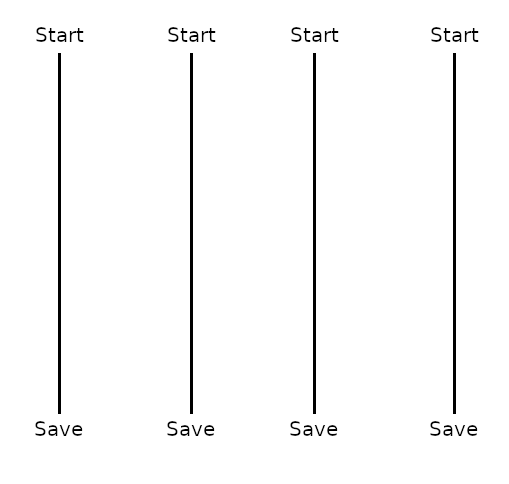
\includegraphics[width=3in]{EmbarsParallel.png}
\item Map-Reduce: data shared between processes\\
- speed-up= $\frac{1}{(1-p)+p/n}$ where p is the fraction of code which is parallelizable and n is the number of cores\\
- harder to do across nodes but not impossible\\
- can be stacked multiple times\\
- must have a wait barrier to wait for all processes to be done before having them communicate to each other\\
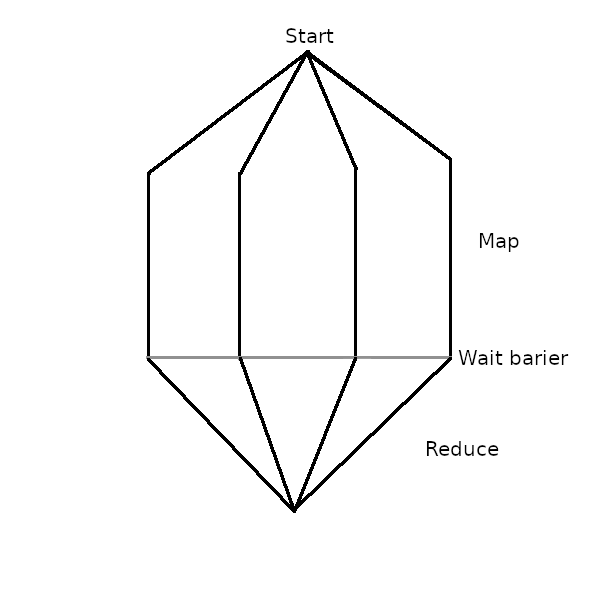
\includegraphics[width=3in]{Map-Reduce.png}
\end{enumerate}
\section{Hyak Structure}

Supercomputers are essentially a collection of high end computers connected via a high speed network that share resources. Each computer is called a node and all nodes share memory and storage.\\
Two types of nodes designed to run code:
\begin{enumerate}
\item Interactive: user has full control using command line
\item Batch: user submits job and node runs without user control
\end{enumerate}
There's also a login node that is designed to only start jobs and manipulate files. All nodes have 28 cores, have access to the entire storage, and have a set partition of memory (can be up to 150 GB).
Nodes are allocated using the slurm scheduler which will give priority based on many parameters including amount of time requested, memory usage, number of nodes, user's history, etc.

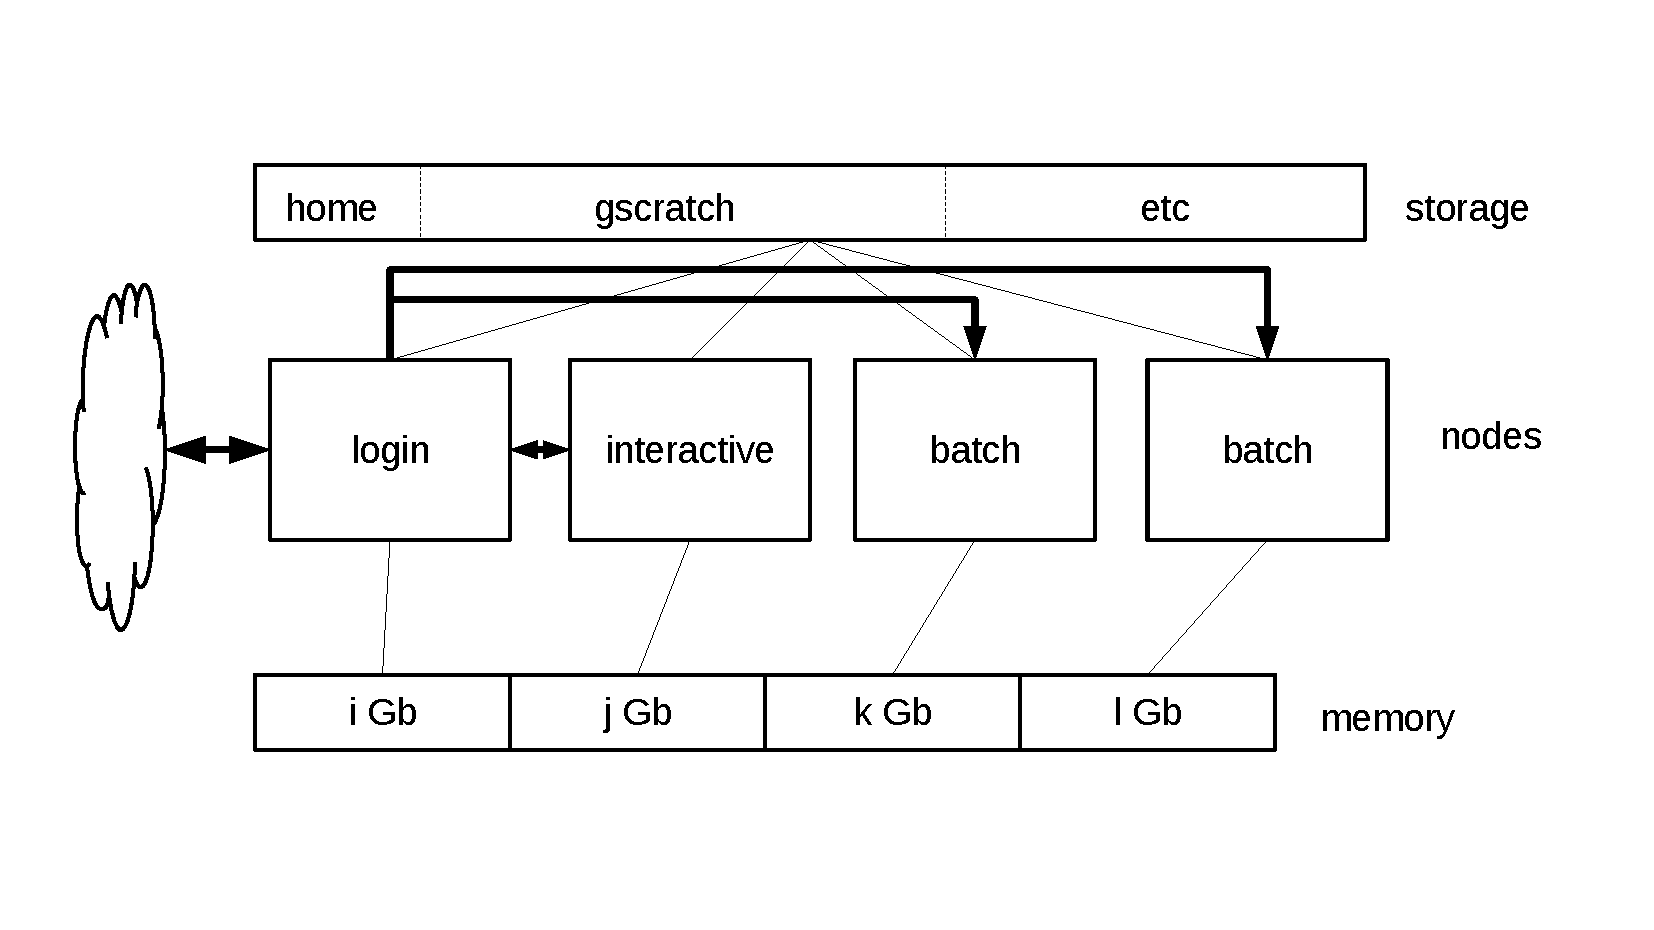
\includegraphics[width=\textwidth]{hyak.pdf}
\section{Useful Commands}
 
\quad\underline{Logging in: gets you into the login node:}
\begin{lstlisting}
ssh username@mox.hyak.uw.edu
\end{lstlisting}

\underline{Get interactive node:}
\begin{lstlisting}
srun -p group --time=time limit --mem=amount of memory 
	-N number of nodes --pty what to do
	
srun -p stf --time=1:00:00 --mem=10GB -N 2 --pty /bin/bash
\end{lstlisting}
stf = student technology fee\\

\underline{To load software:}
\begin{lstlisting}
module load (software name)
\end{lstlisting}

\underline{Submit batch job:}\\

First make script using google or examples then 
\begin{lstlisting}
sbatch myscript.slurm
\end{lstlisting}

\underline{See status of job:}
\begin{lstlisting}
scontrol show job (job #)
\end{lstlisting}
\end{document}